\documentclass{beamer}

\usefonttheme{professionalfonts} % using non standard fonts for beamer
\usefonttheme{serif} % default family is serif

\usepackage{hyperref}
%\usepackage{minted}
\usepackage{animate}
\usepackage{graphicx}
\def\Put(#1,#2)#3{\leavevmode\makebox(0,0){\put(#1,#2){#3}}}
\usepackage{colortbl}
\usepackage{tikz}
\usepackage{amssymb}
\usepackage{enumerate}
\usepackage{arydshln}
\usepackage{algorithm}
\usepackage{algpseudocode}

\colorlet{lightred}{red!25}
\colorlet{lightgreen}{green!25}


\newcommand\blfootnote[1]{%

  \begingroup

  \renewcommand\thefootnote{}\footnote{#1}%

  \addtocounter{footnote}{-1}%

  \endgroup

}

\makeatletter

%%%%%%%%%%%%%%%%%%%%%%%%%%%%%% Textclass specific LaTeX commands.

 % this default might be overridden by plain title style

 \newcommand\makebeamertitle{\frame{\maketitle}}%

 % (ERT) argument for the TOC

 \AtBeginDocument{%

   \let\origtableofcontents=\tableofcontents

   \def\tableofcontents{\@ifnextchar[{\origtableofcontents}{\gobbletableofcontents}}

   \def\gobbletableofcontents#1{\origtableofcontents}

 }

%%%%%%%%%%%%%%%%%%%%%%%%%%%%%% User specified LaTeX commands.

\usetheme{Malmoe}

% or ...

\useoutertheme{infolines}

\addtobeamertemplate{headline}{}{\vskip2pt}

\setbeamercovered{transparent}

% or whatever (possibly just delete it)

\makeatother

\begin{document}
\title[PFLOCK report]{PFLOCK Report}
\author[AC]{Andres Calderon}
\institute[Fall'19]{University of California, Riverside}
\makebeamertitle
\newif\iflattersubsect

\AtBeginSection[] {
    \begin{frame}<beamer>
    \frametitle{Outline} 
    \tableofcontents[currentsection]  
    \end{frame}
    \lattersubsectfalse
}

\AtBeginSubsection[] {
    \begin{frame}<beamer>
    \frametitle{Outline} 
    \tableofcontents[currentsubsection]  
    \end{frame}
}

\begin{frame}{A problem with the time to time approach...}
    \centering
    \begin{tikzpicture}
    \node [anchor=west, scale=0.5] (note) at (2,-1) {Bug!};
    \begin{scope}[xshift=1.5cm]
        \node[anchor=south west,inner sep=0] (image) at (0,0) {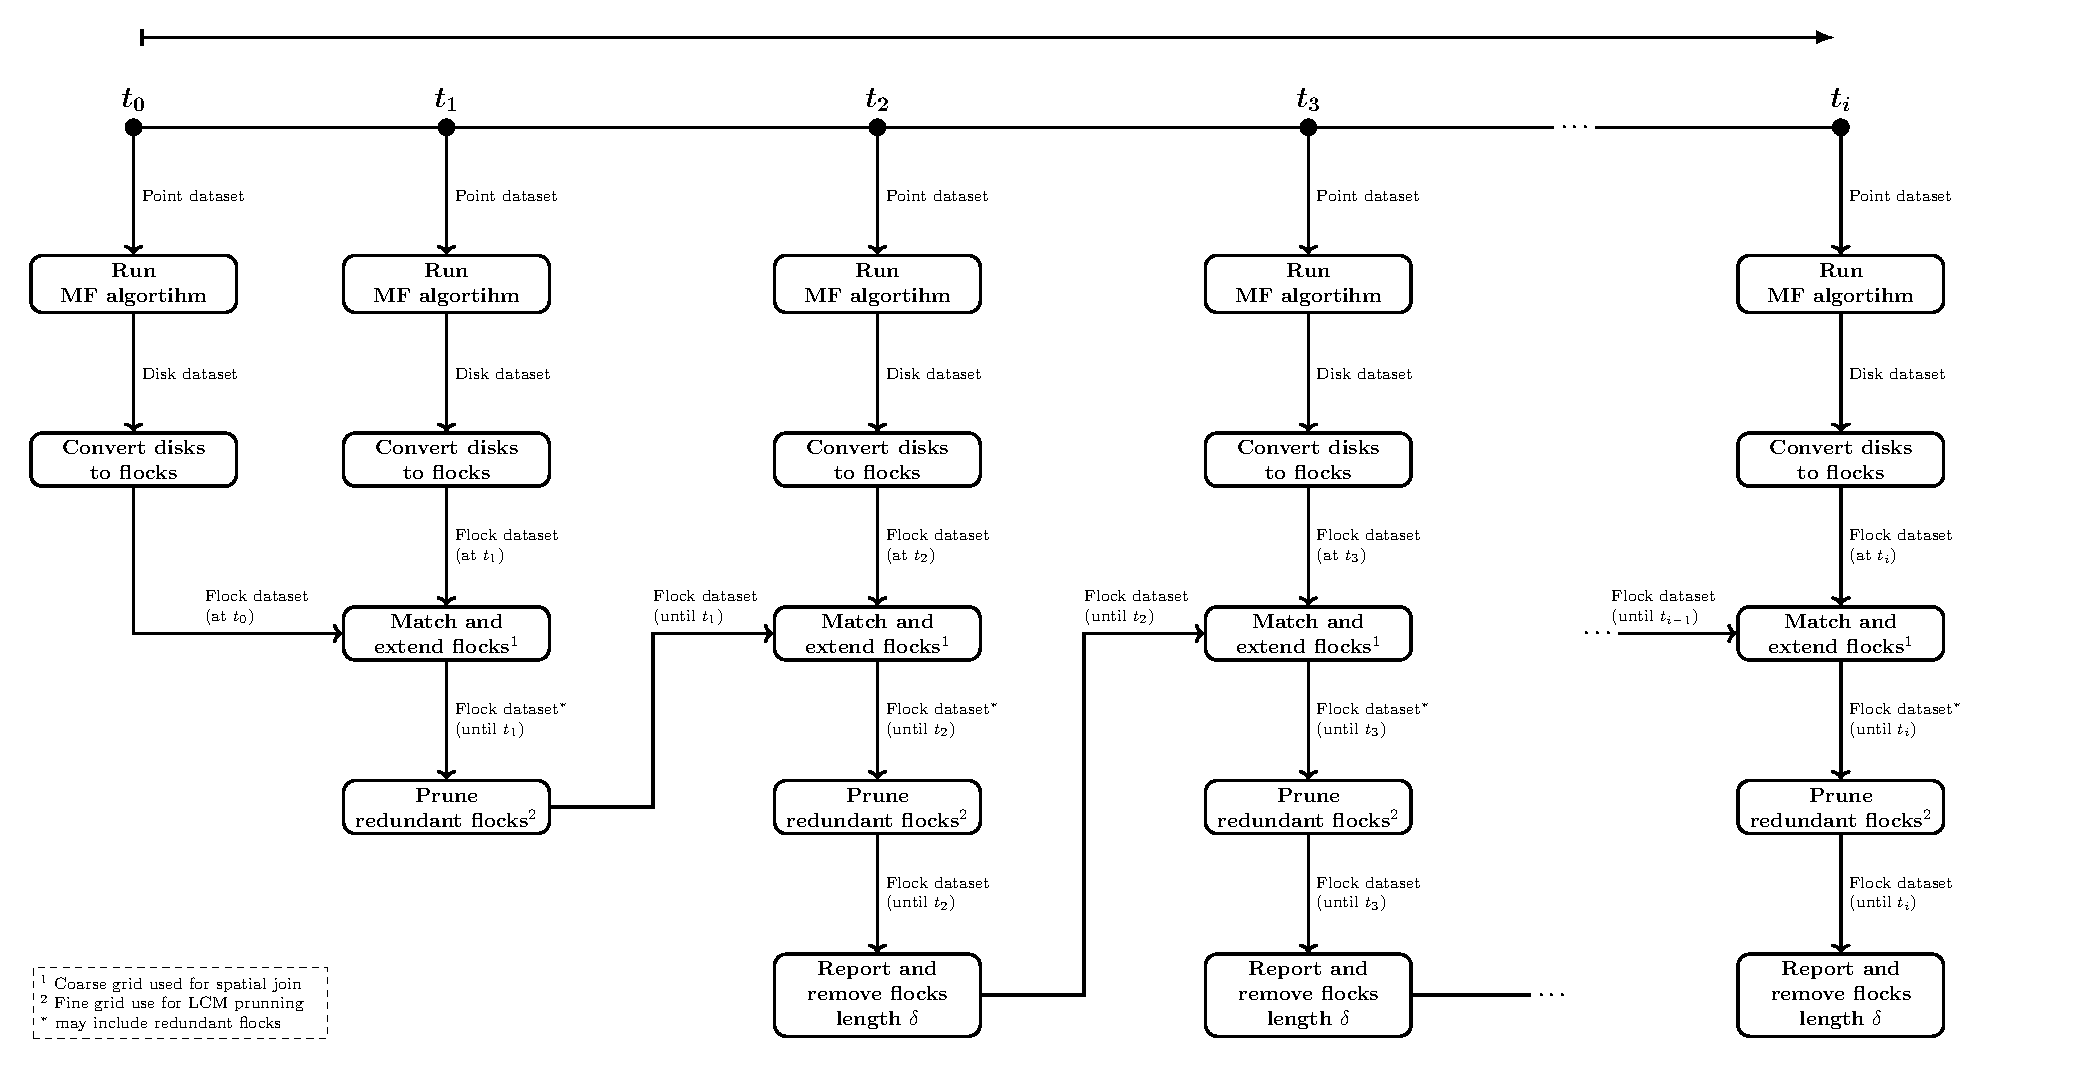
\includegraphics[width=\linewidth]{Figures/FF_flowchart}};
        \begin{scope}[x={(image.south east)},y={(image.north west)}]
            \draw[red,thick,rounded corners] (0.15,0.2) rectangle (0.95,0.29);
            \draw [-latex,thick, red] (note) to[out=0, in=-120] (0.3,0.2);
        \end{scope}
    \end{scope}
    \end{tikzpicture}%
\end{frame}

\begin{frame}{What should ``Prune redundant flocks'' do...}
    \begin{minipage}{.32\textwidth}
        \centering
        \scalebox{0.75}{
            \begin{tabular}{ c c c}
                \multicolumn{3}{c}{\textbf{Current flocks}} \\ \hline
                Start & End & Trajectories \\ \hline
                \rowcolor{lightgreen}
                0 & 1 & A B C D \\
                0 & 1 & A C F \\
                0 & 1 & B F G H \\
                \rowcolor{lightgreen}
                0 & 1 & B H I J \\
                0 & 1 & C E H \\
                & $\vdots$ & \\ \hline
            \end{tabular}
        }
    \end{minipage}%
    \begin{minipage}{0.32\textwidth}
        \centering
        \scalebox{0.75}{
            \begin{tabular}{ c c c}
                \multicolumn{3}{c}{\textbf{New flocks}} \\ \hline
                Start & End & Trajectories \\ \hline
                \rowcolor{lightred}
                1 & 1 & A B C \\
                1 & 1 & A C F I\\
                \rowcolor{lightred}
                1 & 1 & B H I \\
                1 & 1 & D F K \\
                & $\vdots$ & \\ \hline
            \end{tabular}
        }
    \end{minipage}%
    \begin{minipage}{0.32\textwidth}
        \centering
        \scalebox{0.75}{
            \begin{tabular}{ c c c}
                \multicolumn{3}{c}{\textbf{Resulting flocks}} \\ \hline
                Start & End & Trajectories \\ \hline
                0 & 1 & A B C D \\
                0 & 1 & A C F \\
                0 & 1 & B F G H \\
                0 & 1 & B H I J \\
                0 & 1 & C E H \\
                1 & 1 & A C F I\\
                1 & 1 & D F K \\
                & $\vdots$ & \\ \hline
            \end{tabular}
        }
    \end{minipage}
\end{frame}

\begin{frame}{What I did wrong...}
    \begin{minipage}{.32\textwidth}
        \centering
        \scalebox{0.75}{
            \begin{tabular}{ c c c}
                \multicolumn{3}{c}{\textbf{Current flocks}} \\ \hline
                Start & End & Trajectories \\ \hline
                0 & 1 & A B C D \\
                0 & 1 & A C F \\
                0 & 1 & B F G H \\
                0 & 1 & B H I J \\
                0 & 1 & C E H \\
                & $\vdots$ & \\ \hline
            \end{tabular}
        }
    \end{minipage}%
    \begin{minipage}{0.32\textwidth}
        \centering
        \scalebox{0.75}{
            \begin{tabular}{ c c c}
                \multicolumn{3}{c}{\textbf{New flocks}} \\ \hline
                Start & End & Trajectories \\ \hline
                1 & 1 & A B C \\
                1 & 1 & A C F I\\
                1 & 1 & B H I \\
                1 & 1 & D F K \\
                & $\vdots$ & \\ \hline
            \end{tabular}
        }
    \end{minipage}%
    \begin{minipage}{0.32\textwidth}
        \centering
        \scalebox{0.75}{
            \begin{tabular}{ c c c}
                \multicolumn{3}{c}{\textbf{Resulting flocks}} \\ \hline
                Start & End & Trajectories \\ \hline
                0 & 1 & A B C D \\
                \rowcolor{lightred}
                0 & 1 & A C F \\
                0 & 1 & B F G H \\
                0 & 1 & B H I J \\
                0 & 1 & C E H \\
                1 & 1 & A B C \\
                \rowcolor{lightgreen}
                1 & 1 & A C F I\\
                1 & 1 & B H I \\
                1 & 1 & D F K \\
                & $\vdots$ & \\ \hline
            \end{tabular}
        }
    \end{minipage}
\end{frame}

\begin{frame}{A possible solution...}
    \centering
    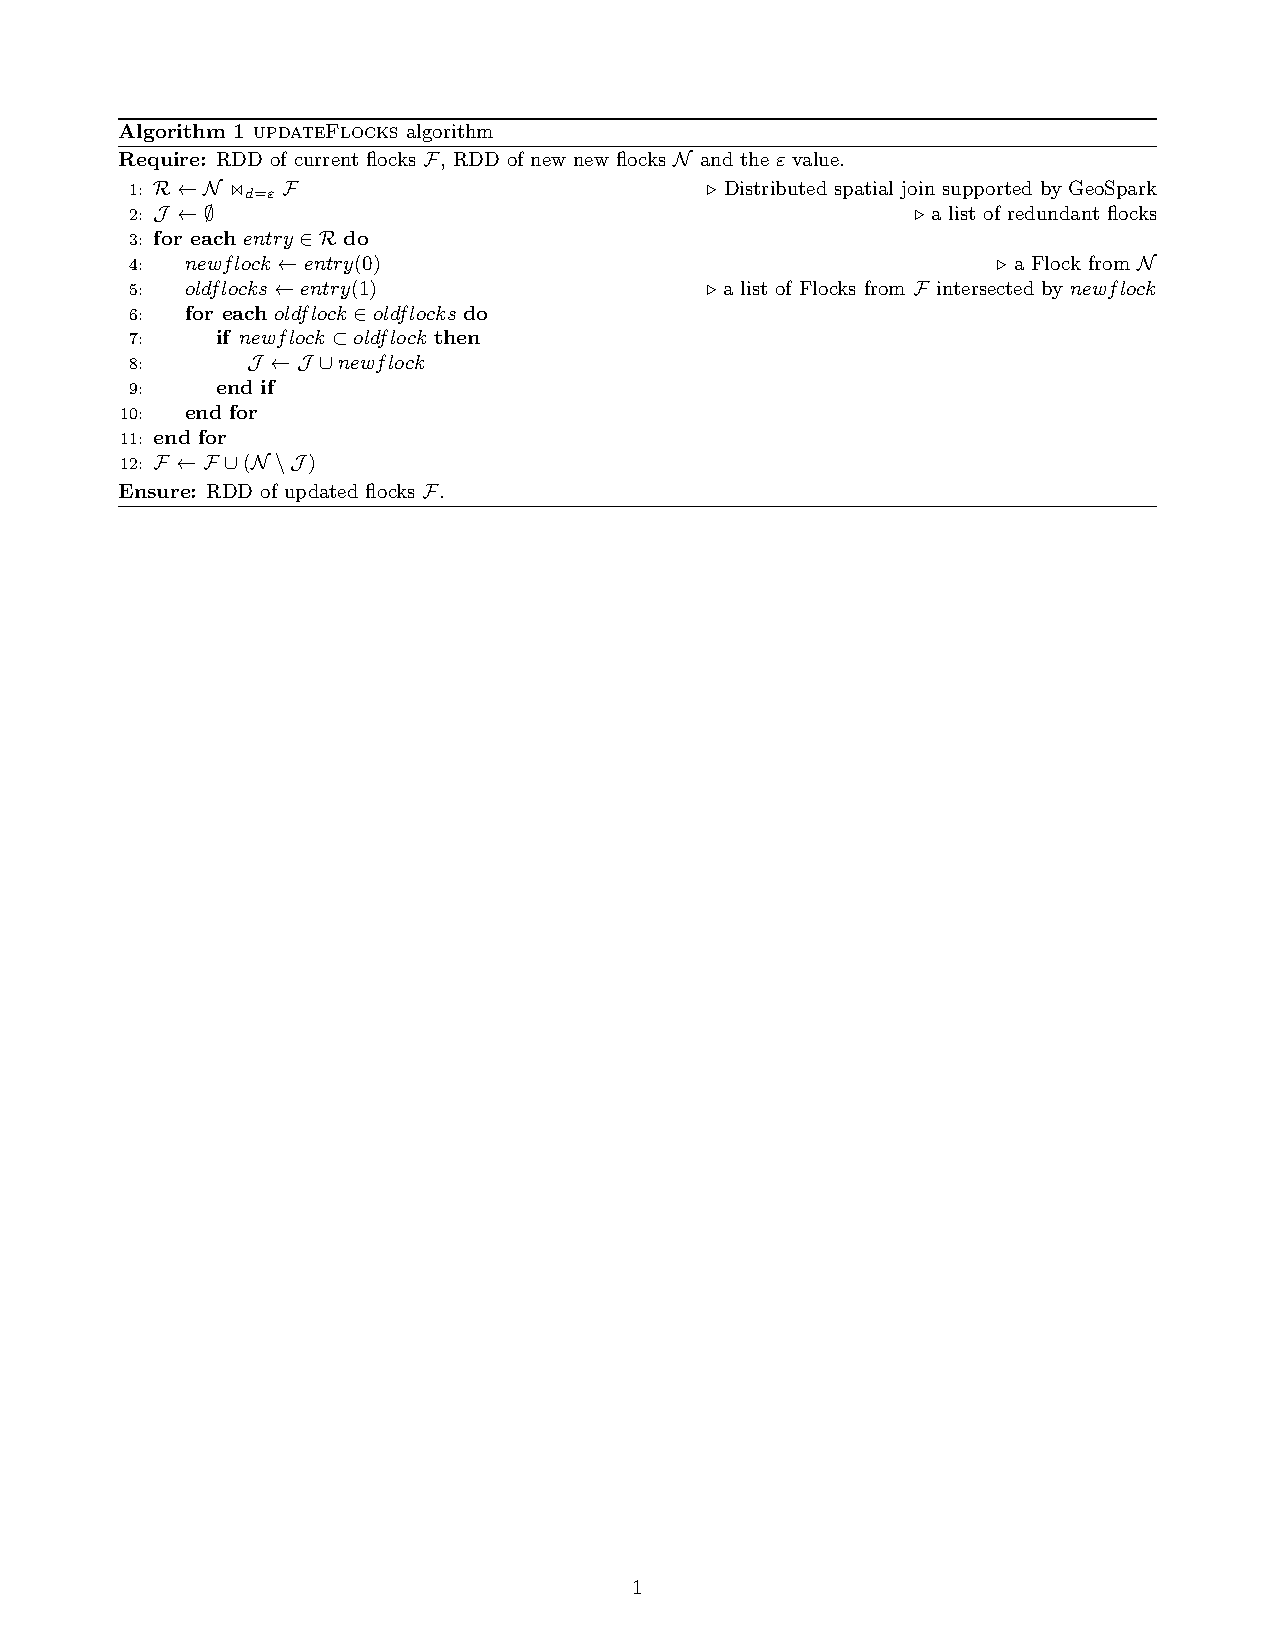
\includegraphics[trim={2cm 10 2cm 2},clip,width=1\linewidth]{Figures/algorithm}
\end{frame}

\end{document}
